\documentclass{report}
\usepackage{tikz}
\usepackage{amsmath}
\usepackage[left=2cm,top=2cm,right=2cm,bottom=2cm]{geometry} 
\usepackage[utf8]{inputenc}
\usepackage[T1]{fontenc}
\usepackage[english]{babel}
\usepackage[document]{ragged2e}


\begin{document}
\begin{titlepage}


    \centering
    {\bfseries\Huge Trabajo \# 4 M\'aximos y minimos \par}
    \vspace{1cm}
    {\Huge Calculo Diferencial }
    \vspace{1cm}
    \vspace{3cm}
    \vspace{3cm}

    {\bfseries\Huge Leocarlos Ospina Causil \par}
    {\bfseries\Huge Moises Doria Lopez \par}
    {\bfseries\Huge Caleb Seña Melo \par}

    \vfill
    {\bfseries\Huge  Diciembre 2022 \par}
\end{titlepage}

{\Large 1.A $ f(x) = 2x^3 -3x^2 -12x + 1, en [-2,3] $ \par}

{\Large\justify

Note que $ 2x^3 -3x^2 -12x + 1$ es continua y por el teorema del valor extremo
tiene un maximo y un minimo absoluto \\
Encontramos los puntos criticos :
\begin{align*}
     & f(x) = 2x^3 -3x^2 -12x + 1 &  &  &  &  &  &  & \\
     & f'(x) = 6x^2 -6x -12
\end{align*}

Veamos cuando $f'(x) = 0$

\begin{align*}                                    
     & 6x^2 -6x -12 = 0                                      &  &  &  &  &  &  & \\
     & x = \frac{ -(-6) \pm \sqrt{(-6)^2 -4(6)(-12)}} {2(6)}                     \\
     & x = \frac{ 6 \pm\sqrt{36 + 288}} { 12}                                    \\
     & x =  \frac{ 6 \pm\sqrt{324}} { 12}                                        \\
     & x = \frac{6\pm18}{12}                                                     \\
     & x1 = \frac {24}{12}                                                       \\
     & x2 = \frac{-12}{12}                                                       \\
     & x1 = 2                                                                    \\
     & x2 = -1
\end{align*}

Ahora evaluamos $f$ en x = 2 y $f$ en x = -1
\begin{align*}
     & f(2) = 2(2)^3 -3(2)^2 -12(2) + 1      &  &  &  &  &  &  &  &  &  &  & \\
     & f(2) = 16 -12 -24 +1 = -19                                                    \\\\
     & f(-1) = 2(-1)^3 -3(-1)^2 -12(-1) + 1                                          \\
     & f(-1) = -2 -3 + 12 +1 = 8                                                     \\\\\\
\end{align*}

\vspace{2cm}
Ahora con -2 y 3

\begin{align*}
     & f(-2) = 2(-2)^3 -3(-2)^2 -12(-2) + 1 &  &  &  &  &  &  &  &  &  &  &  &  &  & \\
     & f(-2) = -16 -12 +24 +1 = -3                                                   \\\\
     & f(3) = 2(3)^3 -3(3)^2 -12(3) + 1                                              \\
     & f(3) = 54 - 27 -36 + 1 = -8
\end{align*}

ahora :\\

\begin{align*}
       f(2) = -19 \\
       f(-1) = 8\\
       f(-2) = -3\\
       f(3) = -8 \\
\end{align*}


Minimo absoluto es $ f(2) = -19 $ y maximo absoluto es $f(-1) = 8 $
}
\vspace{20cm}

{\Large 1.B $ f(x) = 2x^3+ 3x^2 -36x , en [-4,5] $ \par}
{\Large\justify
Note que $  2x^3+ 3x^2 -36x$ es continua y por el teorema del valor extremo
tiene un maximo y un minimo absoluto \\
puntos criticos:
\begin{align*}
     & f(x) = 2x^3 +3x^2 -36x     &  &  &  &  &  &  &  &  &  &  &  &  &  & \\
     & f'(x)= 6x^2 + 6x -36                                                   
\end{align*}
Veamos cuando $f'(x) = 0$
\begin{align*}
     & f'(x)= 6x^2 + 6x -36 = 0   &  &  &  &  &  &  &  &  &  &  &  &  &  &    \\
     & x = \frac{ -(6) \pm \sqrt{(6)^2 -4(6)(-36)}} {2(6)}                     \\
     & x = \frac{ -6 \pm\sqrt{36 + 864}} { 12}                                  \\
     & x =  \frac{ -6 \pm\sqrt{900}} { 12}                                        \\
     & x = \frac{6\pm30}{12}                                                     \\
     & x1 = \frac {-6 + 30}{12} = 2                                                      \\
     & x2 = \frac{ -6 -30}{12} = -3                                                      \\
     & x1 = 2                                                                    \\
     & x2 = -3
\end{align*}
Evamualos en $ x = 2 $ y $ x = -3 $
\begin{align*}
     & f(2) = 2(2)^3 +3(2)^2 -36(2)      &  &  &  &  &  &  &  &  &  &  &  &  &  & \\
     & f(2) = 16 + 12 -72  = -44                                                    \\\\
     & f(-3) = 2(-3)^3 +3(-3)^2 -36(-3)                                           \\
     & f(-3) = -54  + 27 + 108 = 81                                                   \\
\end{align*}
Evamualos en $ a = -4  $ y $ b = 5 $
\begin{align*}
     & f(-4) = 2(-4)^3 +3(-4)^2 -36(-4)      &  &  &  &  &  &  &  &  &  &  &  &  &  & \\
     & f(-4) = -128 + 48 +144  = 64                                                    \\\\
     & f(5) = 2(5)^3 +3(5)^2 -36(5)                                           \\
     & f(5) = 250  + 75 - 180 = 145                                                  \\
\end{align*}
Ahora :\\\\
$  f(-3) = 81 $\\
$  f(2) = - 44$\\
$  f(-4) = 64$\\
$  f(5) = 145 $\\
Minimo absoluto es $ f(2) = -44 $ y maximo absoluto es $ f(5) = 145 $
}

\vspace{20cm}
{\Large 2.  $ f(x) = 4x^3+ 3x^2 -6x +1$ \par}
{\Large\justify
Calculamos la derivada :

\begin{align*}
     & f'(x) = \frac{d }{d x}  \left(  4x^3+ 3x^2 -6x +1  \right)    &  &  &  &  &  &  &  &  &  &  &  &  &  & \\
     & f'(x) = \frac{d}{dx } \left(4x^3 \right) + \frac{d}{dx }\left(3x^2\right)   +\frac{d}{dx}\left(1\right)  \\
     & f'(x) =    12x^2 +6x -6                         \\
     &                                                \\
\end{align*}
Veamos cuando f'(x) = 0
\begin{align*}
     &  12x^2 +6x -6 =  0 &  &  &  &  &  &  &  &  &  &  &  &  &  & \\
     &  \frac{ 12(12x^2 +6x -6)}{12}                                          \\
     & \frac{ (12x^2) + 6(12x-6)}{12}\\
     & (x+1) (12x-6)\\
     & x = -1 & x = \frac{6}{12} =\frac{1}{2} \\
\end{align*}

Aplicamos la ley del cementerio

\begin{tabular}{c c c c }
     (x+1)  & - & + & + \\ 
     (12x-6)& - & - & +\\
            & + & - &  + \\
\end{tabular}

$ f'(x) < 0 $ Cuando X $ \in \left( -\infty,-1 \right) U \left( \frac{1}{2},\infty\right)$\\
\\Entonces:\\\\
F  Decrece en $\left( -\infty,-1 \right) U \left( \frac{1}{2},\infty\right)$\\\\
F Incrementa en $ \left(-1 , \frac{1}{2}\right)$\\
}\\
\vspace{10cm}
{\Large 3.  $ f(x) = x^4 -2x^2 +3 $\par}

{\Large\justify
Calculamos la derivada 

\begin{align*}
     &f'(x) = \frac{d}{dx}\left(x^4 -2x^2 +3\right)&&&&&&&&&&&&&&&&\\
     &f'(x) = \frac{d}{dx}\left(x^4 \right) + \frac{d}{dx}\left(-2x^2\right)+ \frac{d}{dx}\left(3\right)\\
     &f'(x) = 4x^3 -4x  
\end{align*}
 
Factorizamos  y hallamos los puntos criticos
\begin{align*}
     &  4x^3 -4x = 0 &&&&&&&&&&&&&&&&\\
     & 4x(x^2 -1) = 0 \\
     & 4x(x - 1)(x + 1) = 0\\
     & x = 0 , x = 1 ,  x = -1&\\
\end{align*}

Determinamos f'(x) > 0 y f(x) < 0\\\\
\begin{tabular}{c c c c c }
     (4x)    & - & - & + & + \\ 
     (x - 1) & - & - & - & +\\
     (x + 1) & - & + & + & + \\
             & - & + & - & +
\end{tabular}

Tenemos que :\\\\
$ f'(x) < 0 $ Cuando X $ \in  \left(-1,0\right) $ U$ \left(1,+\infty\right)$\\
$ f'(x) > 0 $ Cuando X $ \in  \left(-\infty,1\right) $ U$ \left(0,+1\right)$\\
\\De esto se obtiene:\\\\
$X = -1  $ Es minimo\\
$X =  0  $ Es maximo\\
$X =  1  $ Es Minimo\\

}



\vspace{4cm}
{\Large\justify  4. $f(x) = 6x^4 -8x^3 -24x^2+3$}
\Large\justify{

\begin{align*}
     &f(x) = 6x^4 -8x^3 -24x^2+3\\
     &f'(x) = 24x^3 -24x^2 -48x\\
     &f(x) = 72x^2 -48x - 48\\
\end{align*}

Para poder encontrar los intevalos de concavidad y los puntos de 
inflexion primero necesito los puntos criticos de f''(x) osea que
f''(x) = 0
\begin{align*}
     &f(x) = 72x^2 -48x 48\\
     &24(3x^2 -2x-2)= 0\\
     & 3x^2 -2x-2 = \frac{0}{24}\\
     & 3x^2 -2x-2 = 0\\
\end{align*}

Usamos la formula general
\begin{align*}
     & 3x^2 -2x-2 = 0\\
     & x = \frac{ -(-2) \pm \sqrt{(-2)^2 -4(3)(-2)}} {2(3)}                     \\
     & x = \frac{ 2 \pm\sqrt{4+24}} {6}                                    \\
     & x =  \frac{ 2 \pm\sqrt{28}} { 6}                                        \\
     & x = \frac{2\pm2\sqrt{7}}{6}                                                     \\
     & x1 = \frac {1-\sqrt{7}}{3}                                                       \\
     & x2 = \frac {1+\sqrt{7}}{3}                                                          \\
\end{align*}

\vspace{14cm}
Usamos la ley del sementerio

\begin{tabular}{c c c c  }
     3$x^{2}$ -2x-2  & - & - & + \\ 
     3$x^{2}$ -2x-2  & + & - & + \\
                     & - & + & + 
\end{tabular}

En el intervalo de $\left( -\infty, \frac{1-\sqrt{7}}{3}\right)$ es concava hacia abajo\\
En el intervalo de $\left( \frac{1-\sqrt{7}}{3}, \frac{1+\sqrt{7}}{3}\right)$ es concava hacia arriba\\
En el intervalo de $\left( \frac{1+\sqrt{7}}{3},\infty\right)$ es concava hacia arriba\\

Los puntos de inflexion son $\frac{1-\sqrt{7}}{3}$, $\frac{1+\sqrt{7}}{3}$\\



}

\vspace{30cm}


{\Large 5.  $ f(x) =  x^2(6-x)^3 $\par}
\Large\justify{
     Calculamos $f'(x)$

     \begin{align*}
          &f(x) =  x^2(6-x)^3&&&&&&&&&&&&&&&&&&&&\\
          &f'(x) = \frac{d}{dx}\left( x^2(6-x)^3 \right) \\
          &f'(x) = \frac{d}{dx}\left(6-x^3 \right)  x^2 +(6-x)^3 \frac{d}{dx}\left(x^2\right) \\
          &f'(x) = 3(6-x)^2(0-1)x^2 + (6-x)^3x^2\\
          &f'(x) = 2(6-x)^2 x-3(6-x)^2x^2   \\
          &f'(x) = -(6-x)^2 x(5x-12) \\
     \end{align*}
     
     Ahora Calculamos la segunda derivada
     \begin{align*}
          &f'(x) =   -(6-x)^2 x(5x-12) &&&&&&&&&&&&&&&&&&&&\\
          &f''(x) =  -\left(\frac{d}{dx}(x-6)^2 x \left(5x-12\right)+\left(x-6\right)^2 \frac{d}{dx}\left(x\right) \left(5x-12\right) +\left(x-6\right)^2x\frac{d}{dx}\left(5x-12\right)\right)\\
          &f''(x) =  -2(x-6)(1+0)x(5x-12)-(x-6)^2(5x-12)-5(x-6)^2x\\
          &f''(x) =  -2(x-6)x(5x-12)-(x-6)^2(5x-12)-5(x-6)^2x\\
          &f''(x) =  (x^2 +12x)(5x-12)(-x+6)^2(5x-12)(-5x^2 +30x)^2  \\
          &f''(x) =  5x^3+12x^2+60x-144x(-x+6)(-x+6)(5x-12)(-5x^2+30x)^2 \\
          &f''(x) =  5x^3 +12x^2-84x-5x^2+12x+30x-72(-x+6)(-5x^2 +30x)^2\\
          &f''(x) = -20x^3 + 216x^2-648x+432
     \end{align*}

     Buscamos los puntos criticos 

     \begin{align*}
          &f'(x) = -(x-6)^2(x)(5x-12) = 0&&&&&&&&&&&&&\\
          & -(x-6)^2 x (5x-12) = 0  \\\\
          & -(x-6)^2 = 0 &&   x = 0 && 5x-12=0\\
          & (x-6 )=0  && x = 0&& 5x = 12\\
          & x = 6  && x = 0 &&x = \frac{12}{5}\\
     \end{align*}

     \vspace{6cm}
     X = 6\\
     X = 0\\
     X = $\frac{12}{5} $\\

     Evaluar f''(x) con cada punto critico
     \begin{align*}
          &f''(6) = -20(6)^3 + 216(6)^2-648(6)+432 &&&&&&&&&&&&&\\
          & f''(6) =  -4320 + 7776 -3888 + 432 = 0\\
     \end{align*}
     No hay informacion de maximos o minimos en $f''(6)$
     \begin{align*}
          &f''(0) = -20(0)^3 + 216(0)^2-648(0)+432 &&&&&&&&&&&&&\\
          & f''(0) =  0  + 0 + 432 = 432\\
     \end{align*}

     \begin{align*}
          &f'' \left(\frac{12}{5}  \right)= -20\left(\frac{12}{5}  \right)^3 + 216\left(\frac{12}{5}  \right)^2-648\left(\frac{12}{5}  \right)+432 &&&&&&&&&&&&&\\
          &f'' \left(\frac{12}{5}  \right)=  -\frac{6912}{25}  + \frac{31104}{25} - \frac{7776}{5}+ 432 = -\frac{3888}{25} \\
     \end{align*}
     
     Obtuvimos que \\
     $f''(0) = 0 $ No hay informacion \\
     $f''(6) = $ 432 > 0, hay un Minimo\\
     $f''\left(\frac{12}{5}\right) = - \frac{3888}{25} < 0$ hay un maximo
\\\\
     Aplicamos la regla del cementero  ala primera derivada debido a que no hay informacion
     en $f''(6)$\\
     Ley del cementerio\\

     \begin{tabular}{c c c c c}
          -(x-6)$^{2}$ & - & - & - & -\\ 
          (x)  & - & + & + & +\\
           (5x-12)& - & - &  + &+ \\
           & - & + & - & -\\
     \end{tabular}\\\\
     De esto se deduce que \\
     $x =6 $ No correponde a un maximo o un minimo \\
     $x = 0 $ es un Minimo\\
     $x = \frac{12}{5} $ es maximo

}



{\Large\justify  6A.\\\\ Las dimenciones de la caja corresponden a: ancho  = X , altura = Y , largo = X }

\vspace{1cm}

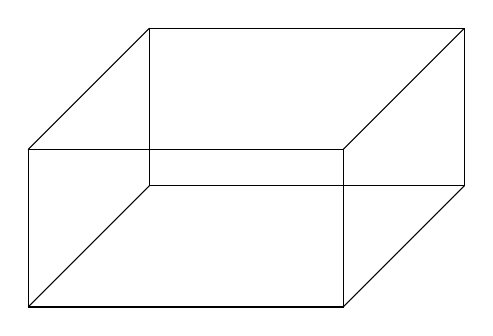
\begin{tikzpicture}
    \draw (0,0,0) -- (4,0,0) -- (4,2) -- (0,2,0) -- cycle;
    \draw (0,0,4) -- (4,0,4) -- (4,2,4) -- (0,2,4) -- cycle;
    \draw (0,0,0) -- (0,0,4);
    \draw (4,0,0) -- (4,0,4);
    \draw (4,2,0) -- (4,2,4);
    \draw (0,2,0) -- (0,2,4);
\end{tikzpicture}

\vspace{1cm}
{\Large

    Usamos la ecuacion del volumen y luego despejamos a Y
    \begin{align*}
         & V = x \cdot x \cdot y &  &  &  &  &  &  &  &  & \\
         & 32000 = x^2 \cdot y
         & y = \frac{32000}{x^2}
    \end{align*}

    Usamos la ecuacion del area y reemplazamos a Y
    \begin{align*}
         & A = 4x y + x^2                                  &  &  &  &  &  &  &  &  &  & \\\\
         & A = 4x \left(    \frac{32000}{x^2}\right) + x^2                              \\\\
         & A = \frac{128000 x}{ x^2 }+ x^2                                              \\\\
         & A = \frac{128000 }{ x }+ x^2
    \end{align*}

    Teniendo la ecuacion del area procedemos a calcular la derivada
    \begin{align*}
         & A = 128000x^{-1} + x^2                                               &  &  &  &  &  &  &  &  &  & \\\\
         & A' =\dfrac {\mathrm{d} }{\mathrm{d} x}\left(128000x^{-1} +x^2\right)                              \\\\
         & A' = -128000x^{-2} + 2x                                                                           \\
    \end{align*}
    La igualamos a 0 y despejamos  x

    \begin{align*}
         & -128000x^{-2} + 2x = 0             &  &  &  &  &  &  &  &  & \\\\
         & 2x = 128000x^{-2}                                            \\\\
         & \frac{2x}{x^{-2}} = 128000                                   \\\\
         & 2x x^{2} = 128000                                            \\\\
         & 2x^{3} = 128000                                              \\\\
         & x^{3} = \frac{128000}{2}                                     \\\\
         & x^{3} = 640000                                               \\\\
         & \sqrt[3]{ x^{3}} = \sqrt[3]{64000}                           \\\\
         & x = 40                                                       \\\\
         & y = \frac{32000}{(40)^2}                                     \\\\
         & y = \frac{32000}{1600}
         & y = 20                                                       \\\\
    \end{align*}

    Las dimenciones de la cajas son $$ X = 40cm  $$  $$Y = 20cm $$
    \begin{flalign*}
    \end{flalign*}





    {\Large\justify  6B.}
    Tenos la presion sanguinea dada por: \\ 

    $f(x) = \frac{1}{2}x^2(k-x) $
    Calculamos la derivada\\
    \begin{align*}
     &= \frac{d}{dx}\left( \frac{1}{2}x^2(k-x) \right)\\
     &= \frac{1}{2}\frac{d}{dx}\left((k-x)x^2\right)\\
     &= \frac{\frac{d}{dx} \left(k-x\right) x^2 +(k-x)\frac{d}{dx}(x^2)}{2}\\
     &= \frac{\left(\frac{d}{dx} (k) -\frac{d}{dx} (x) \right) x^2 +(k-x) 2x}{2}\\
     &= \frac{(0-1)x^2 + (k-x) 2x}{2}\\
     &= (k-x)x -\frac{x^2}{2}\\
     &= kx-x^2 - \frac{x^2}{2}\\
     &= kx \frac{-2x^2-x^2}{2}\\
     &= kx -\frac{3x^2}{2}\\
     \end{align*}
 
     Ahora la igualamos a  0
     \begin{align*}
          &kx -\frac{3x^2}{2}= 0\\
          &x \left( k -\frac{3x}{2} \right)= 0\\
          & k -\frac{3x}{2} = 0\\
     \end{align*}
     Puntos criticos
     \begin{align*}
          x  = 0\\
          x = \frac{2k}{3}\\
     \end{align*}
     Se evalúa con los puntos encontrados
     \begin{align*}
          & f'(x) = xk -\frac{3}{2}x^2\\
          &f''(x) = k -3x \\
          &f''(0) = k \geq 0 0 \\
          &f''\left(\frac{2}{3}k\right)= k -3 \left(\frac{2}{3}k\right)\\
          & = k-2k = -k < 0\\
     \end{align*}

     $f''(x) < 0$ Por lo que hay un punto maximo local en x = $\frac{2k}{3} $

     Evaluamos la funcion inicial con los puntos encontrados

     \begin{align*}
         & f\left(\frac{2k}{3}\right) =\left(\frac{1}{2}\right) \left(\frac{4k^2}{9} \right) \left(\frac{1k}{3}\right)  = \frac{4k^3}{54}  =\frac{2k^3}{27} \geq 0
     \end{align*}

     
     
}



\end{document}